% Capítulo 7: um vetor de 5 elementos, seus índices e a posição que não existe.
\documentclass[border=4pt]{standalone}
\usepackage[utf8]{inputenc}
\usepackage[T1]{fontenc}
% Estilo comum das figuras de vetores (capítulo 8).
\usepackage{tikz}
\usetikzlibrary{arrows.meta, positioning, calc, decorations.pathreplacing}
\definecolor{navy}{RGB}{23,45,80}
\definecolor{laranja}{RGB}{250,110,29}
\definecolor{cinzalogo}{RGB}{107,114,126}
\definecolor{azul}{RGB}{205,222,247}
\tikzset{
  casa/.style={draw=navy, line width=0.9pt, minimum width=8mm, minimum height=7mm,
               inner sep=0pt, font=\sffamily\small},
  pronta/.style={casa, fill=azul},
  parte/.style={casa, fill=laranja!12},
  marcada/.style={casa, fill=laranja!45, draw=laranja},
  fora/.style={casa, draw=cinzalogo!60, dashed, fill=white, text=cinzalogo!60},
  indice/.style={font=\sffamily\scriptsize, text=cinzalogo},
  explica/.style={font=\sffamily\small, text=navy, anchor=east},
  legenda/.style={font=\sffamily\scriptsize, text=cinzalogo},
  rotulo/.style={font=\sffamily\small\bfseries, text=navy},
  seta/.style={-{Stealth[length=2.2mm]}, navy, line width=0.9pt},
  chave/.style={decorate, decoration={brace, amplitude=4pt, mirror}, navy, line width=0.8pt},
}
% \vetor{nome}{x}{y}{valor/estilo, valor/estilo, ...}: casas lado a lado, chamadas nome0, nome1...
\newcommand{\vetor}[4]{%
  \foreach \valor/\estilo [count=\i from 0] in {#4} {
    \node[\estilo] (#1\i) at ($(#2, #3) + (\i*0.8, 0)$) {\valor};
  }
}

\tikzset{casa/.append style={minimum width=11mm, minimum height=8mm}}
\begin{document}
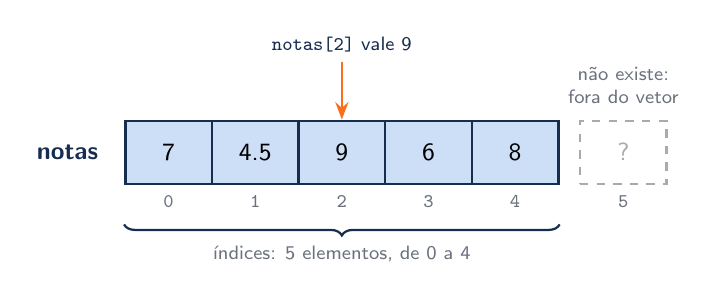
\begin{tikzpicture}[x=11mm]
  \foreach \v [count=\i from 0] in {7, 4.5, 9, 6, 8} {
    \node[pronta] (c\i) at (\i, 0) {\v};
    \node[indice, font=\ttfamily\scriptsize] at (\i, -0.62) {\i};
  }
  \node[fora] (c5) at (5.25, 0) {?};
  \node[indice, font=\ttfamily\scriptsize] at (5.25, -0.62) {5};
  \node[legenda, align=center] at (5.25, 0.85) {não existe:\\fora do vetor};
  \node[rotulo, anchor=east] at (-0.7, 0) {notas};
  \draw[chave] ($(c0.south west)+(0, -0.5)$) -- node[below=4pt, legenda] {índices: 5 elementos, de 0 a 4} ($(c4.south east)+(0, -0.5)$);
  \draw[seta, laranja] (2, 1.15) -- (c2.north);
  \node[legenda, text=navy, anchor=south] at (2, 1.15) {\texttt{notas[2]} vale 9};
\end{tikzpicture}
\end{document}
